\subsection{Hybrid Entropy}
\label{ssec:hybrid-sec}

As mentioned in Section \ref{sssec:hybrid-section}, the Hybrid Entropy equation is as follows:

\begin{equation}
  H_{hy} = -p_0\log(1 - E_0) - p_1\log(E_1)
\end{equation}

Where $E_0$ and $E_1$ can be defined as:

\begin{subequations} \label{eq:E0-E1}
  \begin{align}
    &E_0 = \frac{1}{n}\displaystyle\sum_{i=1}^{n}{(1-\mu_i)exp(\mu_i)} \\
    &E_1 = \frac{1}{n}\displaystyle\sum_{i=1}^{n}{\mu_iexp(1-\mu_i)}
  \end{align}
\end{subequations}

And $p_0$ and $p_1$ are the probabilities of receiving 0 and 1 symbols respectively.

%==============================================================================
\subsubsection{MATLAB implementation}
%==============================================================================

Due to reasons covered in the Subsubsection \ref{sssec:hyrid-technical}, Hybrid Entropy membership was implemented using 2 trapeziums covering 2 fuzzy sets, as seen in Figure

\begin{figure}[H]
  \center
  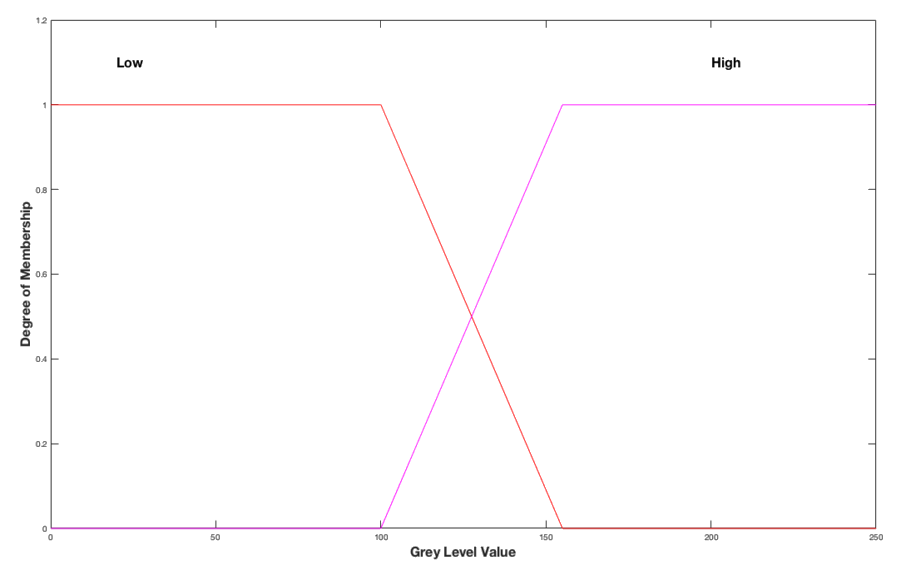
\includegraphics[scale=0.5]{Chapter2/hybrid-img/2_traps.png}
  \caption{Two membership trapeziums for Hybrid Entropy - Low and High grey-level values.}
  \label{fig:2-traps}
\end{figure}

Two arrays are then fed into the Hybrid Entropy function - one listing all the pixel membership values from the low trapezium, and the other from the high trapezium. The final entropy is taken as a comparison between the low and high fuzzy sets.

%==============================================================================
\subsubsection{Technical challenges}
\label{sssec:hyrid-technical}
%==============================================================================

Whilst Hybrid Entropy utilises a membership function, much like Non-Probabilistic entropy, it was derived to work with binary entropy, not the ternary membership modeled for Non-Probabilistic. Because of the binary nature, the equation uses `inversion' to depict if not this fuzzy set, then must belong to the other.

Experimentation was done as to whether the equation could be adapted in such a way to continue using three separate membership trapeziums - low, medium and high grey-level values.

\textbf{Initial ideas - check email between me and neil}


Logic would dictate that if the comparison of two fuzzy sets works, then to compare the low fuzzy set to the medium, the medium to the high and the high to the medium should work.

For example:

\begin{figure}[!ht]
  \centering
  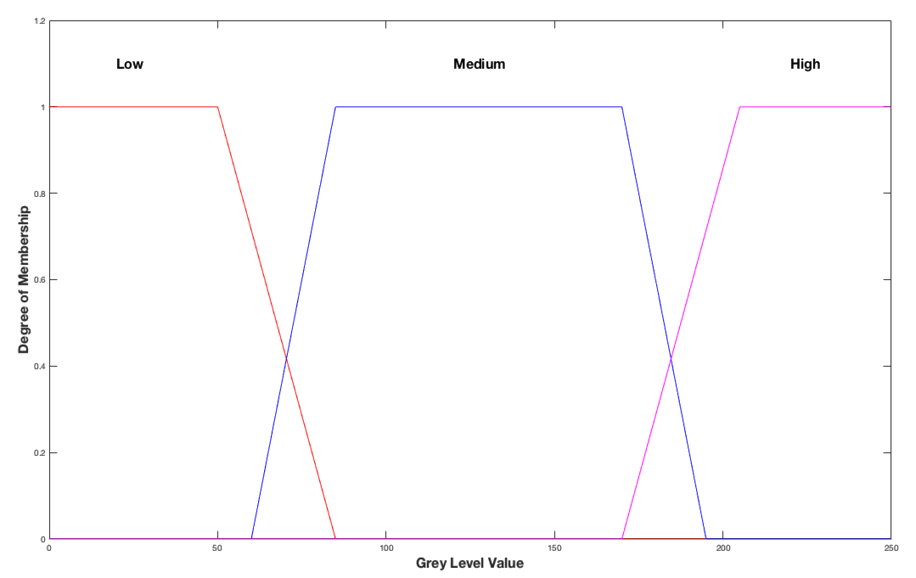
\includegraphics[scale=0.5]{Chapter2/hybrid-img/3_traps.png}
  \caption{3 fuzzy set trapeziums}
  \label{fig:3-traps}
\end{figure}

In theory, calculating $E_0$ and $E_1$ for each trapezium, calculating the hybrid entropy for each, and then combining them, should work:

\begin{equation}
E_0 = \frac{1}{No.\_of\_pixels\_in\_low\_trapezium}\displaystyle\sum_{i=1}^{n}{(1-Low\mu_i)exp(Low\mu_i)}
\end{equation}
\begin{equation}
E_1 = \frac{1}{No.\_of\_pixels\_in\_low\_trapezium}\displaystyle\sum_{i=1}^{n}{Low\mu_iexp(1-Low\mu_i)}
\end{equation}

Where $Low\mu$ is the membership of the pixels in the low fuzzy set.
%http://tex.stackexchange.com/questions/112238/how-to-wrap-a-long-equation-in-latex
\begin{equation}
H_{hy} = -p_0\log_{10}(1 - E_0) - p_1\log_{10}(E_1)
\end{equation}

Where

$p_0 = \frac{No.\_of\_pixels\_in\_low\_trapezium}{No.\_of\_pixels\_in\_low\_trapezium + med\_trapezium}$

and

$p_1 = \frac{No.\_of\_pixels\_in\_med\_trapezium}{No.\_of\_pixels\_in\_low\_trapezium + med\_trapezium}$


This was done for all 3 trapeziums, then combined and divided by 3 (for the mean entropy). As the result for each trapezium should be between 0 and 1 (as each is an entropy value), then combining them should be no issue. However this was not the case.

First of all, the hybrid equation output was deemed to be `NaN' - something which generally occurs when attempting to divide by 0. Anomalous outputs from the high trapezium was to be expected, as there are very few pixels which fall within the range nearer the white end of the grey-level scale. This was mitigated by setting the output equal to 0, in effect ignoring any output from the highest fuzzy set.

After this mitigation, the third and fourth iteration had suitable entropy values, however the fifth entropy value was a negative, something which is not possible in terms of entropy, as it must be between 0 and 1 - see Figure \ref{fig:minus-entropy}.

\begin{figure}[H]
  \begin{center}
  %  \pgfplotsset{every axis/.append style={thick},width=0.4*\textwidth, ymax=1}
  %    \begin{tikzpicture}
  %        width = 10cm,
  %        axis lines = middle,
  %        xlabel = {Iterations},
  %        ylabel = {Entropy},
  %        ymin = -0.3,
  %        ymax = 0.3,
  %        ytick={-0.5,-0.4,...,0.6},
  %        y tick label style={
  %                /pgf/number format/.cd,
  %                fixed,
  %                fixed zerofill,
  %                precision=1,
  %            /tikz/.cd
  %        },
  %        xtick={1,2,...,5},
  %        x label style={at={(axis description cs:0.5,0.3)},anchor=north},
  %        y label style={at={(axis description cs:-0.1,.5)},rotate=90,anchor=south},
  %        nodes near coords,
  %    	  nodes near coords align={vertical},
  %        every node near coord/.append style={font=\scriptsize,
  %                xshift = +3pt, yshift=+4pt,anchor=west, /pgf/number format/precision=6},
  %        ]
  %      \addplot coordinates
  %        { (1, 0.124512) (2, 0.048099) (3, 0.238875) (4, 0.232505) (5, -0.140011) };
  %        \draw[ultra thin] (axis cs:0,\pgfkeysvalueof{/pgfplots/ymin}) -- (axis cs:0,\pgfkeysvalueof{/pgfplots/ymax});
  %      \end{axis}
  %    \end{tikzpicture}
    \end{center}
    \caption{Graph showing the entropy output after 5 iterations}
    \label{fig:minus-entropy}
\end{figure}

It was concluded that the implementation of three fuzzy sets within Hybrid Entropy would not be realistic within the remaining timeframe of the project, and the membership for Hybrid Entropy was redefined to the concept of 2 fuzzy sets, as set out by Pal and Pal. This would mean, one trapezium for pixel grey-level values with low values, overlapping with a high grey-level value trapezium at approximately 128, as seen in Figure \ref{fig:2-traps}.

%==============================================================================
\subsubsection{Run-time}
%==============================================================================
